%%% LaTeX Template: Two column article
%%%
%%% Source: http://www.howtotex.com/
%%% Feel free to distribute this template, but please keep to referal to http://www.howtotex.com/ here.
%%% Date: February 2011

%%% Preamble
\documentclass[	DIV=calc,%
							paper=a4,%
							fontsize=12pt,%
							onecolumn]{scrartcl}	 					% KOMA-article class

\usepackage{lipsum}													% Package to create dummy text
\usepackage[brazil]{babel}										% English language/hyphenation
\usepackage[protrusion=true,expansion=true]{microtype}				% Better typography
\usepackage{amsmath,amsfonts,amsthm}					% Math packages
\usepackage[pdftex]{graphicx}									% Enable pdflatex
\usepackage[svgnames]{xcolor}									% Enabling colors by their 'svgnames'
\usepackage[hang, small,labelfont=bf,up,textfont=it,up]{caption}	% Custom captions under/above floats
\usepackage{epstopdf}												% Converts .eps to .pdf
\usepackage{subfig}													% Subfigures
\usepackage{booktabs}												% Nicer tables
\usepackage{fix-cm}													% Custom fontsizes
\usepackage[utf8]{inputenc}
\usepackage[top=2.5cm, bottom=2.5cm, left=2.5cm, right=2.5cm]{geometry}
\usepackage[ddmmyyyy]{datetime}
\usepackage{placeins}
\addto\captionsenglish{
	\renewcommand\tablename{Tabela}
	\renewcommand\figurename{Figura}
} 
 

 
%%% Custom sectioning (sectsty package)
\usepackage{sectsty}													% Custom sectioning (see below)
\allsectionsfont{%															% Change font of al section commands
	\usefont{OT1}{phv}{b}{n}%										% bch-b-n: CharterBT-Bold font
	}

\sectionfont{%																% Change font of \section command
	\usefont{OT1}{phv}{b}{n}%										% bch-b-n: CharterBT-Bold font
	}



%%% Headers and footers
\usepackage{fancyhdr}												% Needed to define custom headers/footers
	\pagestyle{fancy}														% Enabling the custom headers/footers
\usepackage{lastpage}	

% Header (empty)
\lhead{}
\chead{}
\rhead{}
% Footer (you may change this to your own needs)

%% ====================================
%% ====================================
%% mude o rodape  do projeto
%% ====================================
%% ====================================

\lfoot{\footnotesize \texttt{JRT Treinamentos} \textbullet ~Cabemento Estruturado}


\cfoot{}
\rfoot{\footnotesize página \thepage\ de \pageref{LastPage}}	% "Page 1 of 2"
\renewcommand{\headrulewidth}{0.0pt}
\renewcommand{\footrulewidth}{0.4pt}



%%% Creating an initial of the very first character of the content
\usepackage{lettrine}
\newcommand{\initial}[1]{%
     \lettrine[lines=3,lhang=0.3,nindent=0em]{
     				\color{DarkGoldenrod}
     				{\textsf{#1}}}{}}



%%% Title, author and date metadata
\usepackage{titling}															% For custom titles

\newcommand{\HorRule}{\color{DarkGoldenrod}%			% Creating a horizontal rule
									  	\rule{\linewidth}{1pt}%
										}

\pretitle{\vspace{-30pt} \begin{flushleft} \HorRule 
				\fontsize{50}{50} \usefont{OT1}{phv}{b}{n} \color{DarkRed} \selectfont 
				}

%% ====================================
%% ====================================
%% mude o titulo  do projeto
%% ====================================
%% ====================================

\title{Trabalho Cabeamento Estruturado}					% Title of your article goes here

%% ====================================



\posttitle{\par\end{flushleft}\vskip 0.5em}

\preauthor{\begin{flushleft}
					\large \lineskip 0.5em \usefont{OT1}{phv}{b}{sl} \color{DarkRed}}
\author{Julio Cesar Jardim Pereira, Rubens Ussuy Brandão, Tiago Martins Ferreira}  	% Author name goes here


\postauthor{\footnotesize \usefont{OT1}{phv}{m}{sl} \color{Black} 
					\\JRT Treinamentos 								% Institution of author
					\par\end{flushleft}\HorRule}




\date{}																				% No date




%%% Begin document
\begin{document}
\maketitle
\thispagestyle{fancy} 	
\thispagestyle{empty}		% Enabling the custom headers/footers for the first page 
% The first character should be within \initial{}


%% ====================================
%% ====================================
%% mude o resumo  do projeto
%% ====================================
%% ====================================
\initial{E}\textbf{ste projeto tem como objetivo oferecer uma infraestrutura com alta tecnologia de transmissão de dados, disponibilizando a comunicação para a empresa fictícia JRT Treinamentos. Para isso, serão utilizadas normas regulamentadoras como, NBR-14565-2007 e TIA/EIA-568-B e produtos de qualidade afim de oferecer segurança, confiabilidade, crescimento, facilidade de manutenção e gerenciamento futuro pelos profissionais de tecnologia da informação.
}

%% ====================================
\begin{figure}
	\centering
	\includegraphics{utfpr}
\end{figure}

\vspace{3cm}
\centerline{\textit{\textbf{\today}}}

\clearpage
    \renewcommand*\listfigurename{Lista de figuras}
\listoffigures

\renewcommand*\listtablename{Lista de tabelas}
\listoftables


\clearpage
\renewcommand{\contentsname}{Sumário}
\tableofcontents
\clearpage

%% ====================================
%% ====================================
%% Inicio do texto
%% ====================================
%% ====================================
\section{Introdução}
O projeto será realizado para a empresa privada de treinamentos profissionalizantes a JRT Treinamentos. Temos como objetivo ofertar o serviço de cabeamento estruturado (dados e voz). Utilizando padrões dentro das normas estabelecidas de cada elemento na rede, para uma futura certificação da mesma. O prédio em questão terá 2 pisos que serão interligados através de cabeamento horizontal ligado ao armário de telecomunicações que se interconectam por um backbone.


\subsection{Benefícios}

Com a utilização de normas regulamentadoras e produtos de qualidade poderemos entregar um projeto que vise:
\begin{itemize}
	\item Crescimento.
	\item Facilidade de manutenção e gerenciamento futuro.
	\item Interligação dos andares por meio de fibra óptica para evitar interferências eletromagnéticas.
	\item Pontos lógicos identificados para facilitar na identificação e manutenção da rede.
	\item Cabeamento estruturado para fornecer voz e dados com alta performance.
\end{itemize}

\section{Requisitos}
O projeto a ser realizado deverá fornecer um ponto de dados e voz para cada local onde existe uma mesa que possa ter um colaborador atuando, e contara a principio com 14 pontos de dados e 14 pontos para voz para o piso 1 e 10 pontos de dados e 10 pontos de voz para o piso 2.\newline
Todo o cabeamento estruturado deverá ser implementado respeitando as normas que tratam desse assunto.

\section{Usuários e Aplicativos}
Os usuários vão fazer uso de aparelhos de telefone IP, e cada mesa listada na planta vai ter um computador e um telefone IP para utilização, o plano de ampliação da empresa inclui a criação de laboratórios de informática para cursos na área de TI, os cursos serão oferecidos no futuro.
 

\subsection{Usuários}
Atualmente a JRT Treinamentos conta com um total de 15 colaboradores sendo 2 secretárias, 1 gerente, 3 telefonistas, 2 técnicos de TI e 7 professores.

\subsection{Aplicativos}
Atualmente a empresa conta com 3 servidores virtuais sendo 1 servidor de arquivos com Windows Server 2016, um servidor Active Directory também com Windows Server 2016, e um servidor PABX com Asterisk rodando em sistema operacional Debian 9, todas as máquinas virtuais se encontrão em um unico servidor físico com o Hypervisor XenServer.


\section{Planta Lógica - Elementos estruturados}

\subsection{Estado atual}
A construção conta com a seguinte estrutura atualmente, 6 salas no piso 1 onde dessas 6 salas 5 delas contarão com infraestrutura de dados e voz, e no piso 2 conta com 9 salas onde 4 delas contarão com infraestrutura de dados e voz.\newline
Ambos os pisos contam com estrutura para passagem do cabeamento, como eletrocalhas, canaletas, dutos e caixas de passagem. As Figuras \ref{planta_p1} e \ref{planta_p2} exemplificam as plantas dos pisos 1 e 2 já com a disposição dos pontos.
Para realizar as distribuições dos pontos foi utilizado o software Dutotec que trabalha em conjunto com o AutoCad.

\begin{figure}
	\centering
	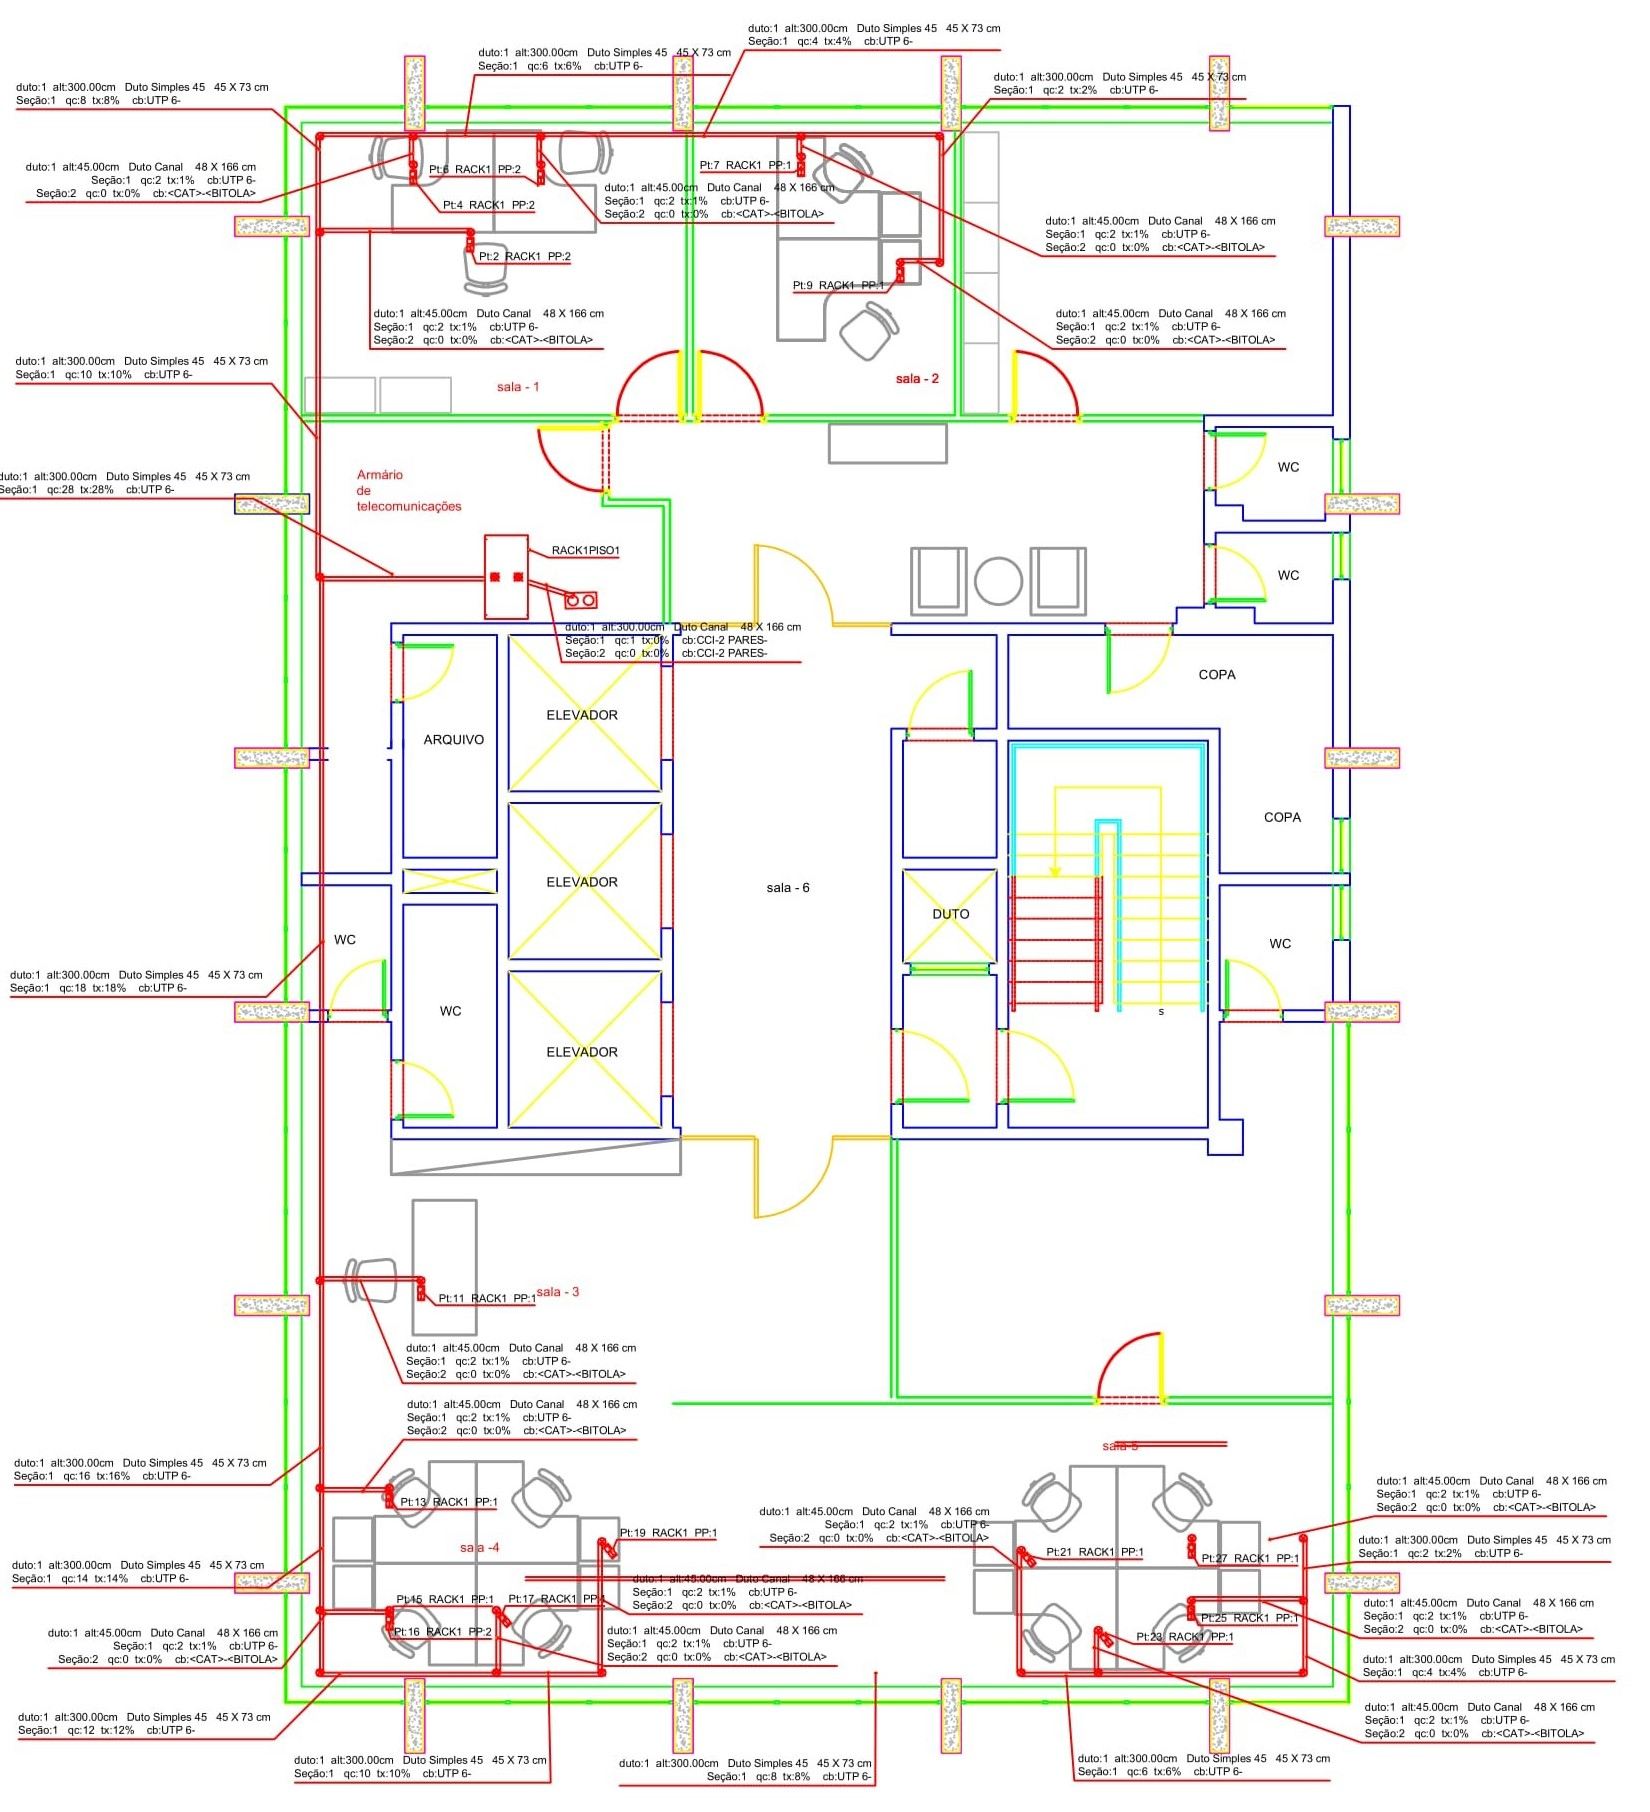
\includegraphics[width=\textwidth]{planta_p1}
	\caption{Planta Piso 1}
	\label{planta_p1}
\end{figure}
\FloatBarrier

\begin{figure}
	\centering
	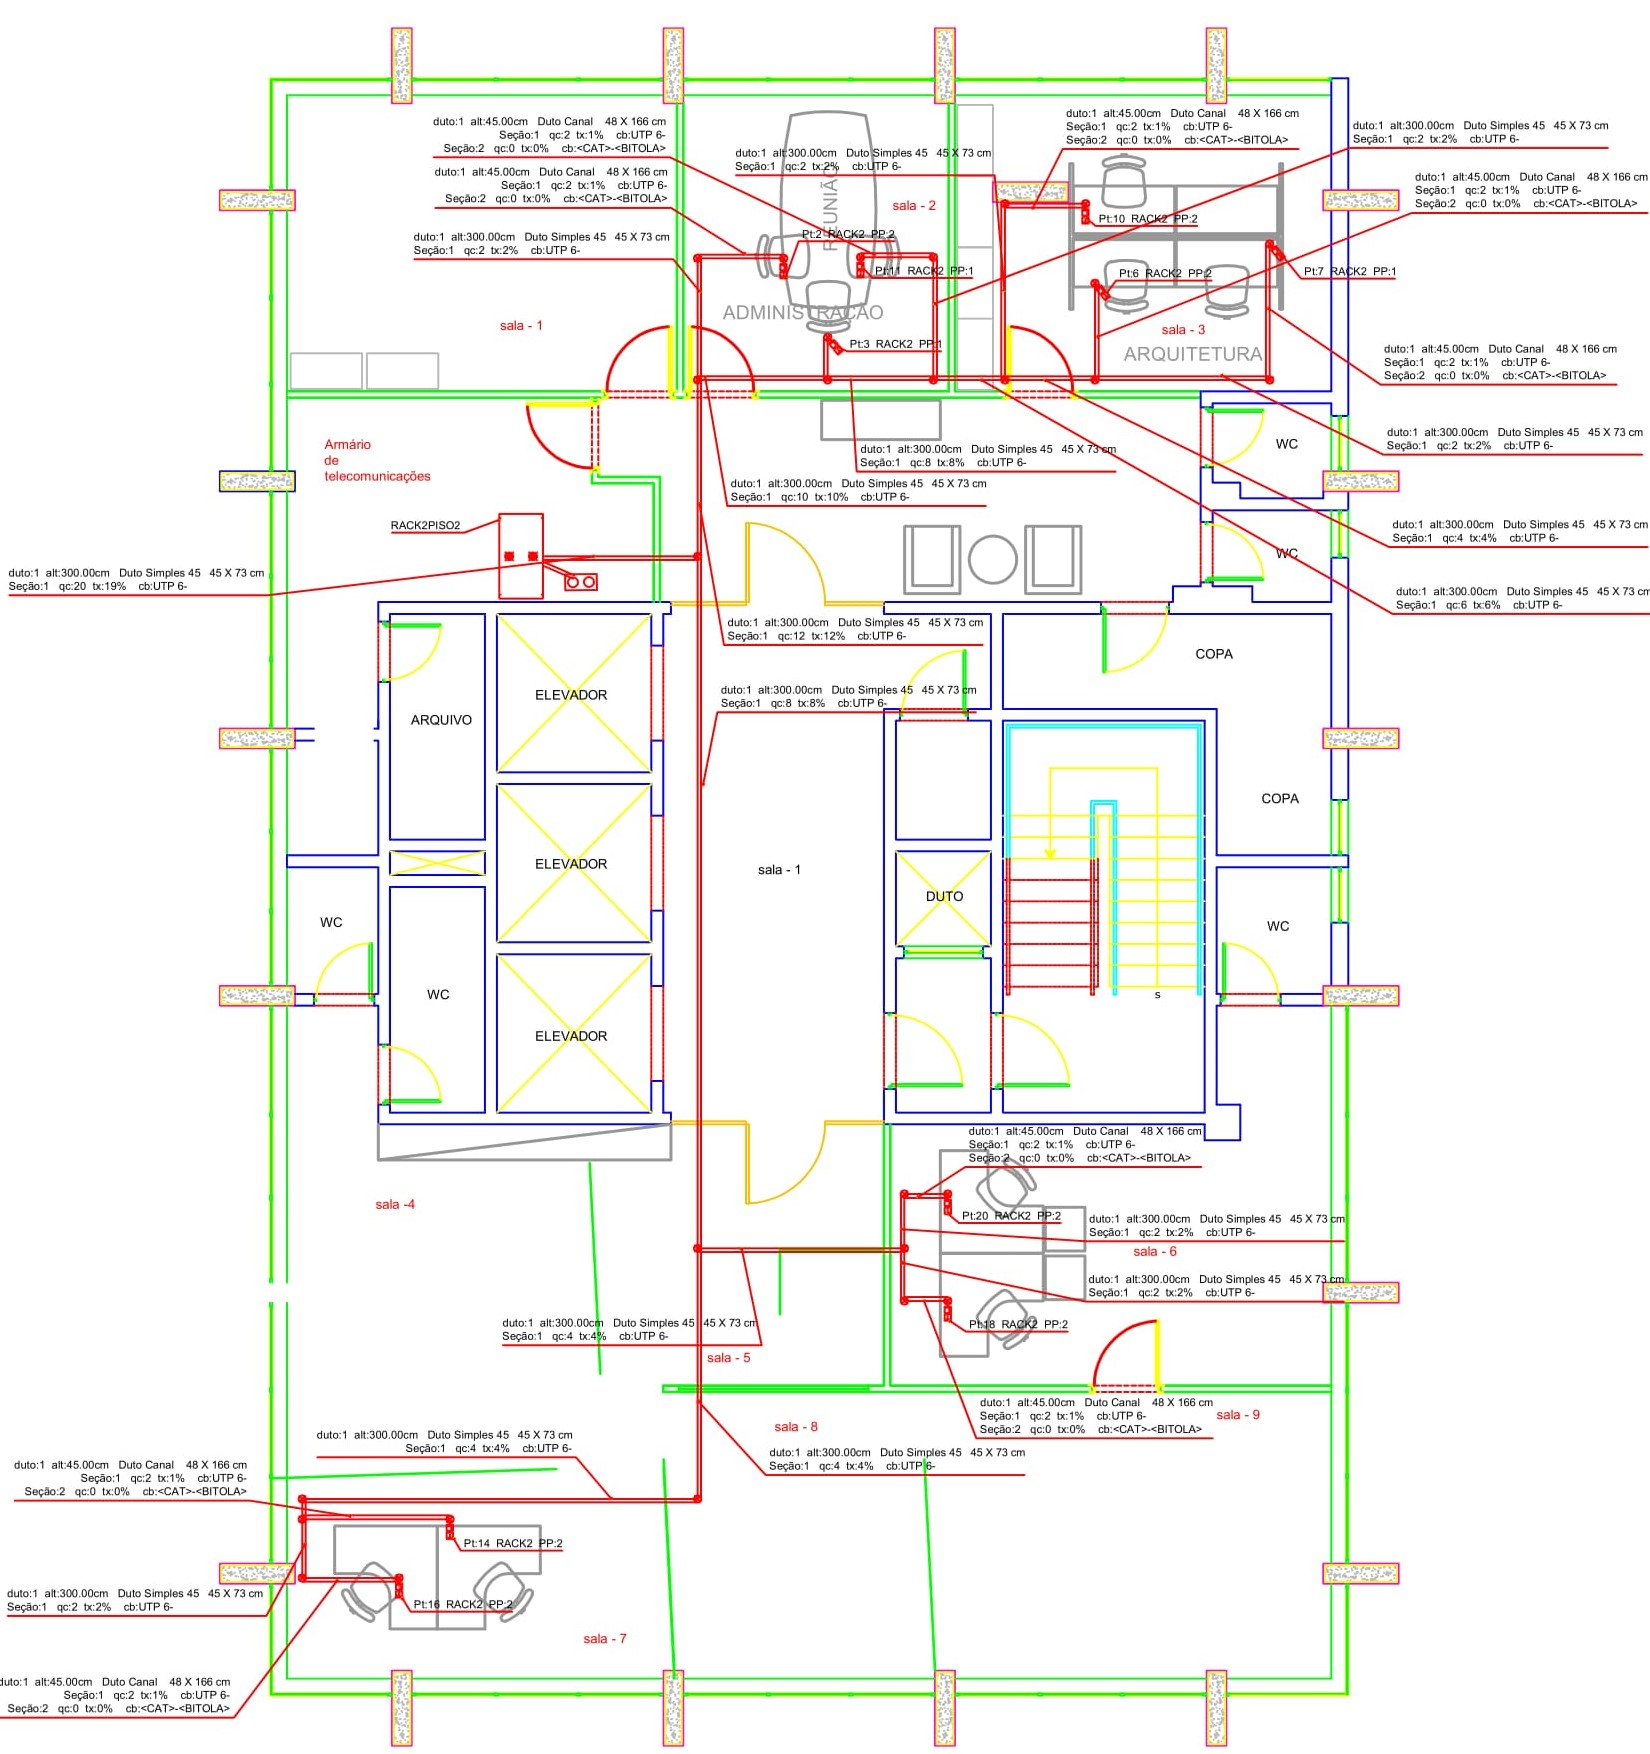
\includegraphics[width=\textwidth]{planta_p2}
	\caption{Planta Piso 2}
	\label{planta_p2}
\end{figure}
\FloatBarrier

\subsection{Topologia}
O layout do cabeamento horizontal se dá na topologia estrela, onde cada ponto de utilização está conectado ao concentrador de forma individual, evitando assim um blackout na rede. Para ligação dos pontos serão utilizados cabos UTP 6 acomodados em eletrocalhas aparentes suspensas a 3 metros do chão. A tomadas de telecomunicações serão instaladas a 45 cm do chão.
O Backbone é feito através de fibra óptica para evitar gargalos no tráfego entre um pavimento e o outro. Apesar da modularidade oferecida pela disposição da rede, os switches foram empilhados afim de melhorar o compartilhamento entre os equipamentos, sendo assim, o switch de dados do pavimento 1 esta empilhado com o switch de dados do pavimento 2, o que faz com que os equipamentos se comportem como se fossem um. O mesmo acontece com o switch destinado a Telefonia.
Os Racks dos dois pisos contam com dois patch panels de 24 portas cada um, também conta com dois switchs gerenciáveis de 24 portas cada, são destinados um patch panel e um switch de cada rack para voz e um patch panel e um switch de cada rack para dados.
As figuras \ref{rack_p1} e \ref{rack_p2} demonstram como ficaram organizados os racks nos dois pisos.\newline
A figura \ref{diag_log} demostra como os racks dos dois pisos se interconectam.

\begin{figure}
	\centering
	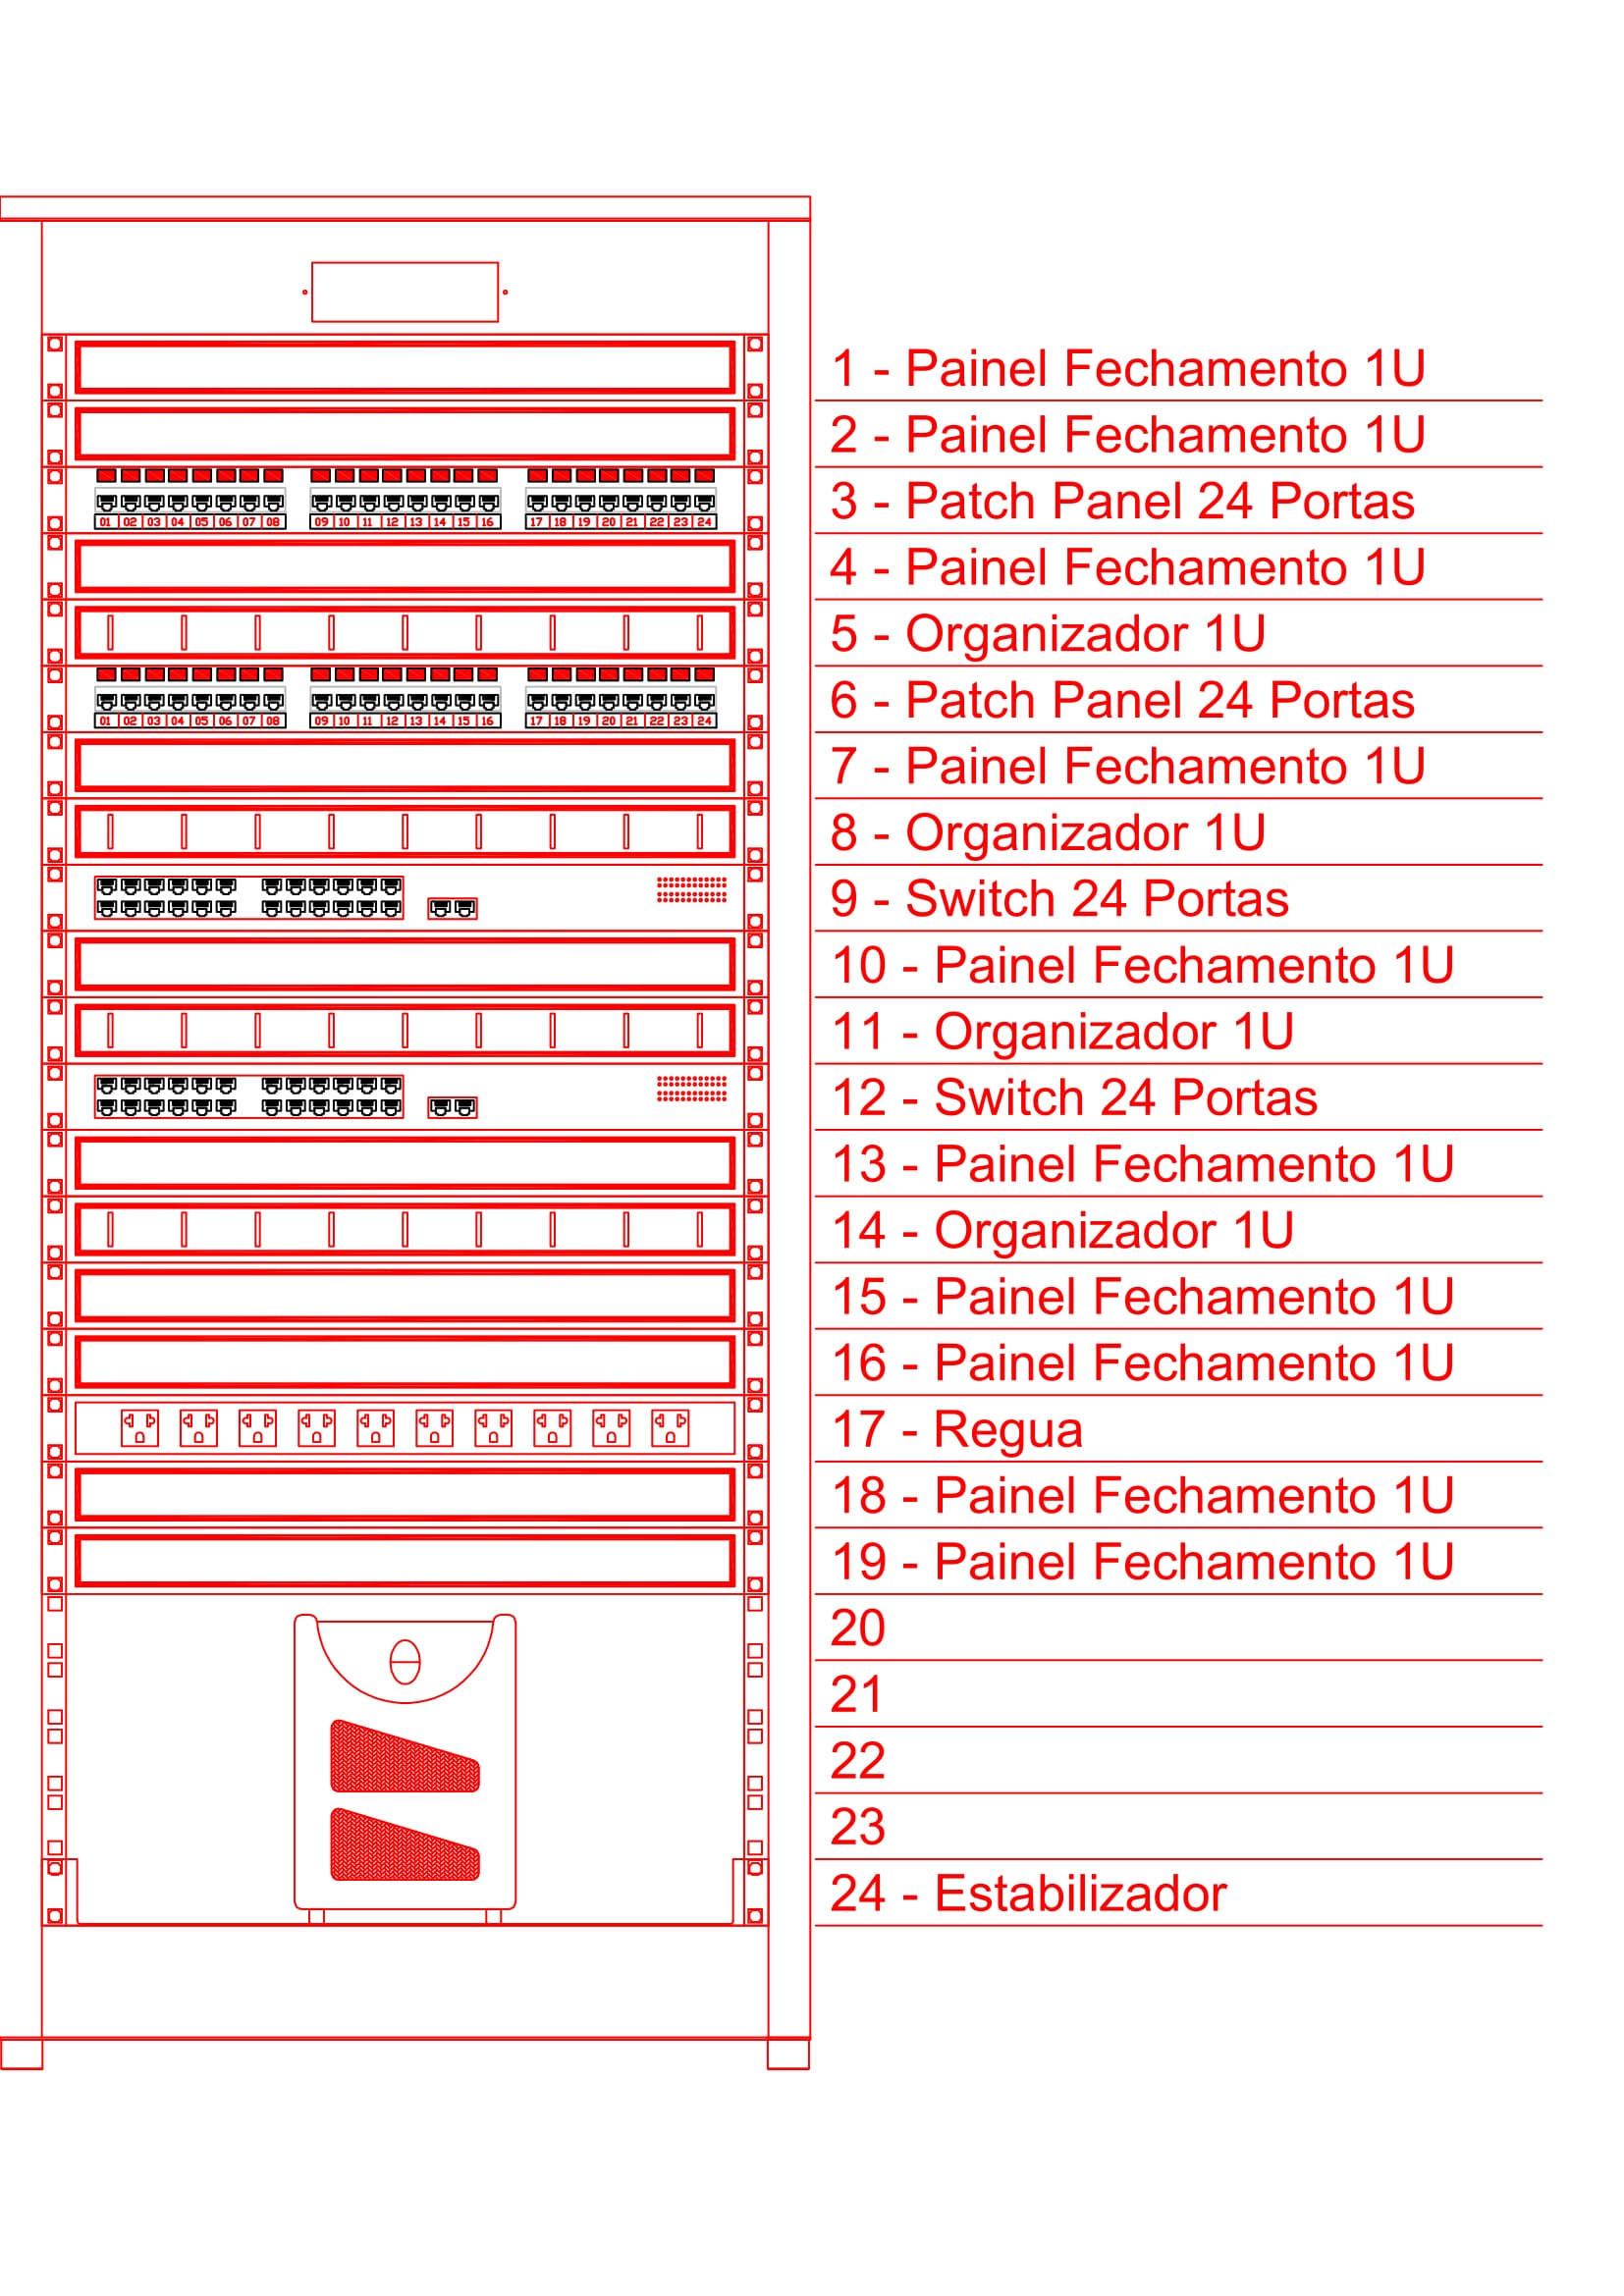
\includegraphics[width=\textwidth]{rack_p1}
	\caption{Rack Piso 1}
	\label{rack_p1}
\end{figure}
\FloatBarrier

\begin{figure}
	\centering
	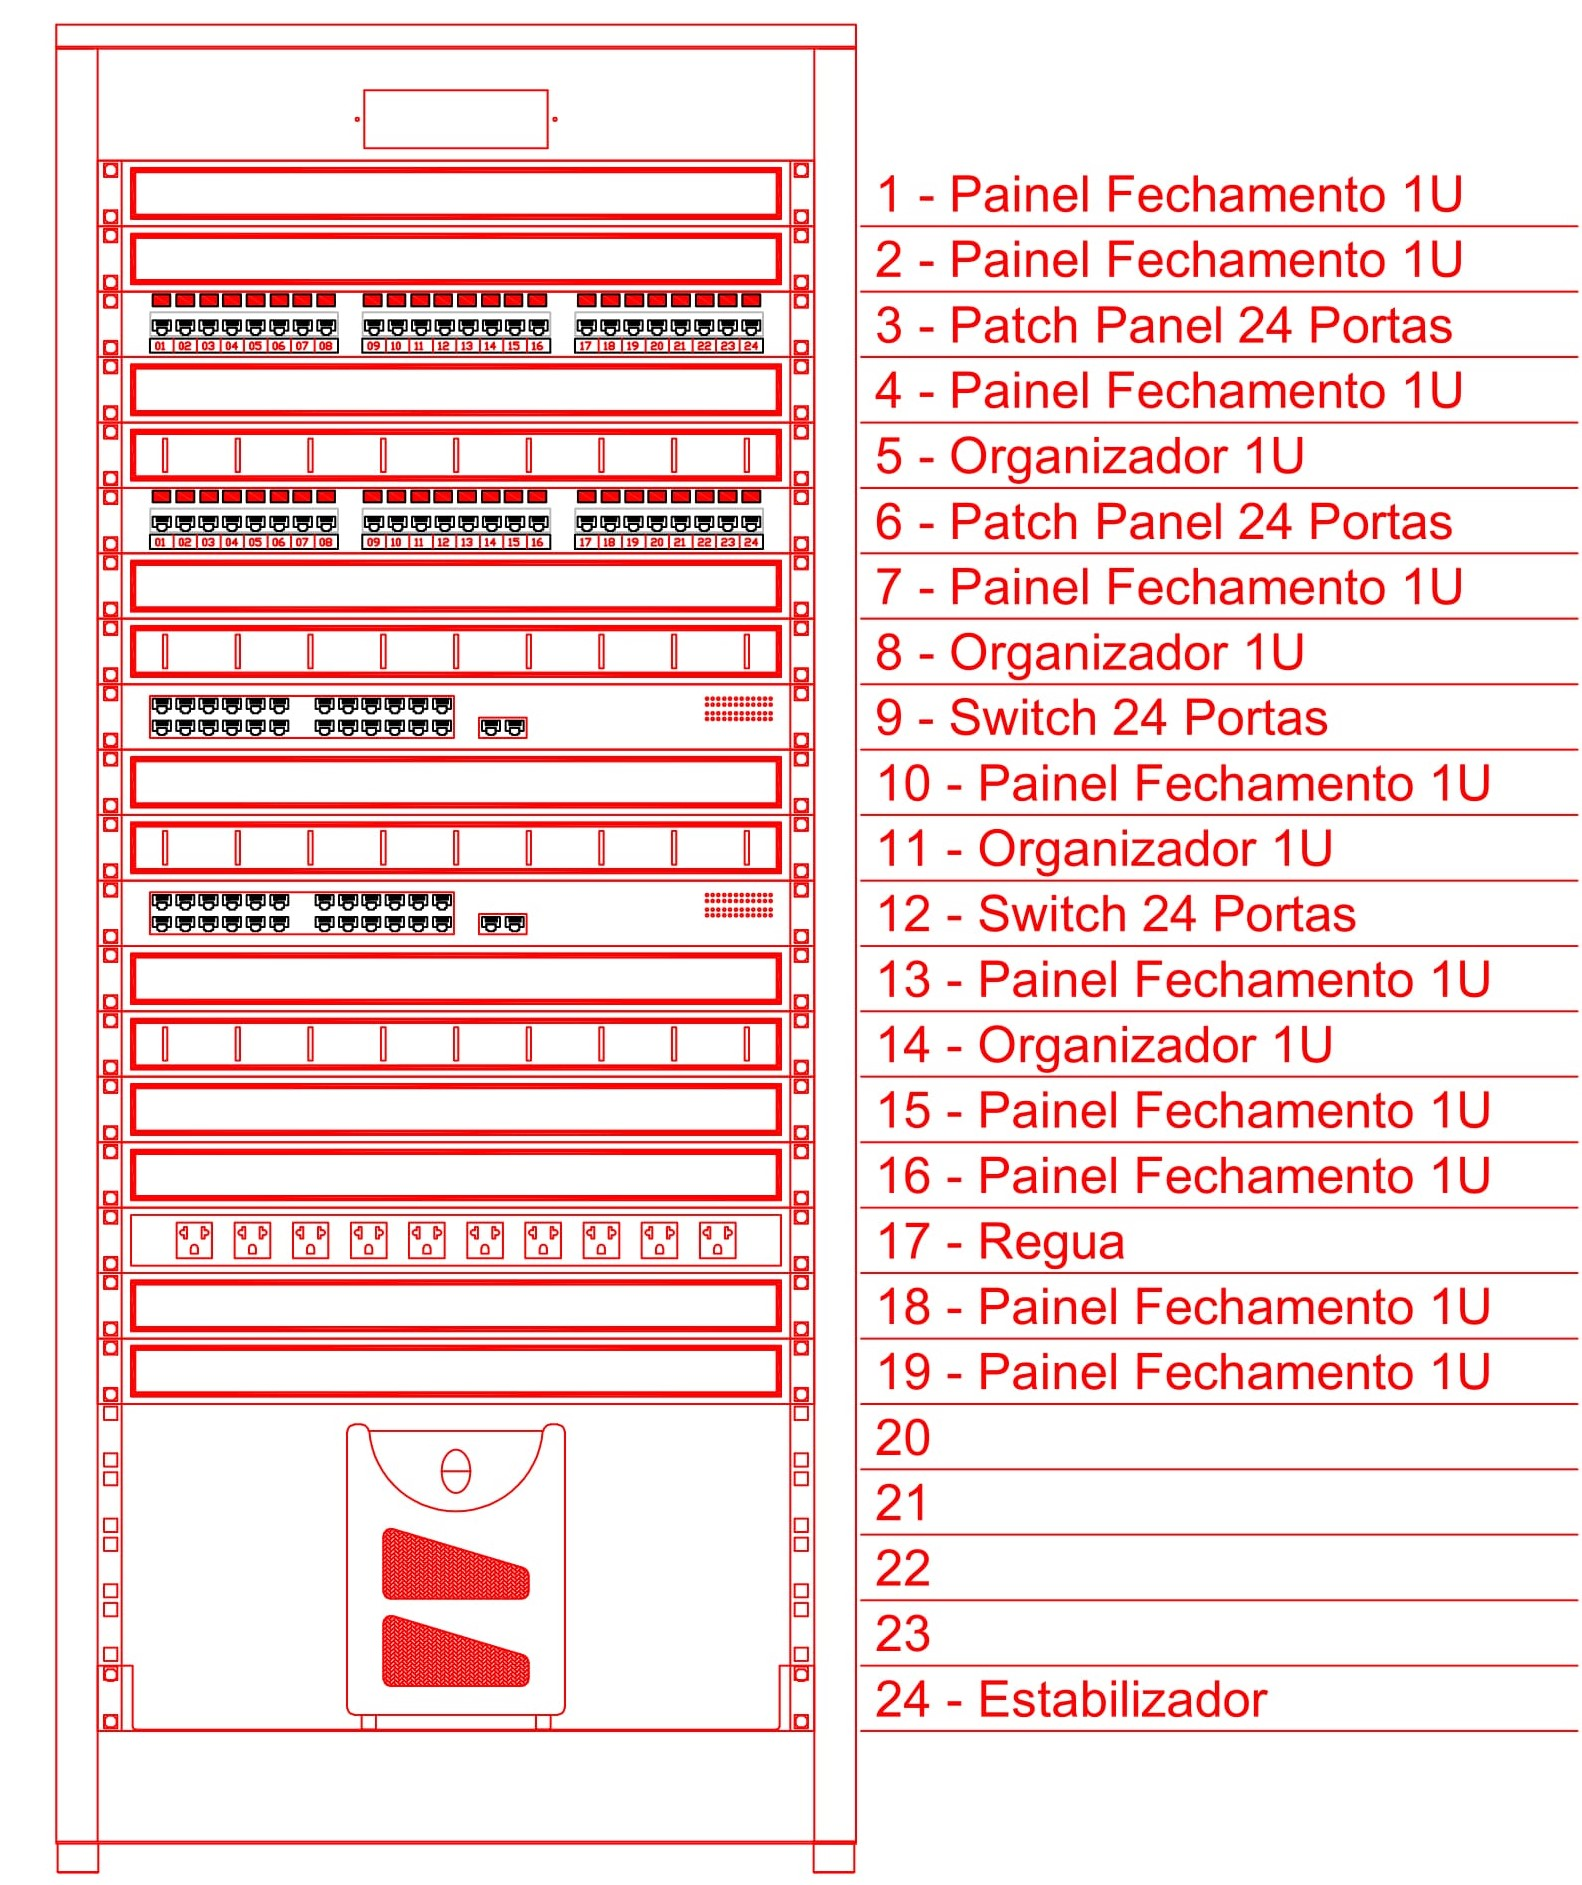
\includegraphics[width=\textwidth]{rack_p2}
	\caption{Rack Piso 2}
	\label{rack_p2}
\end{figure}
\FloatBarrier

\begin{figure}
	\centering
	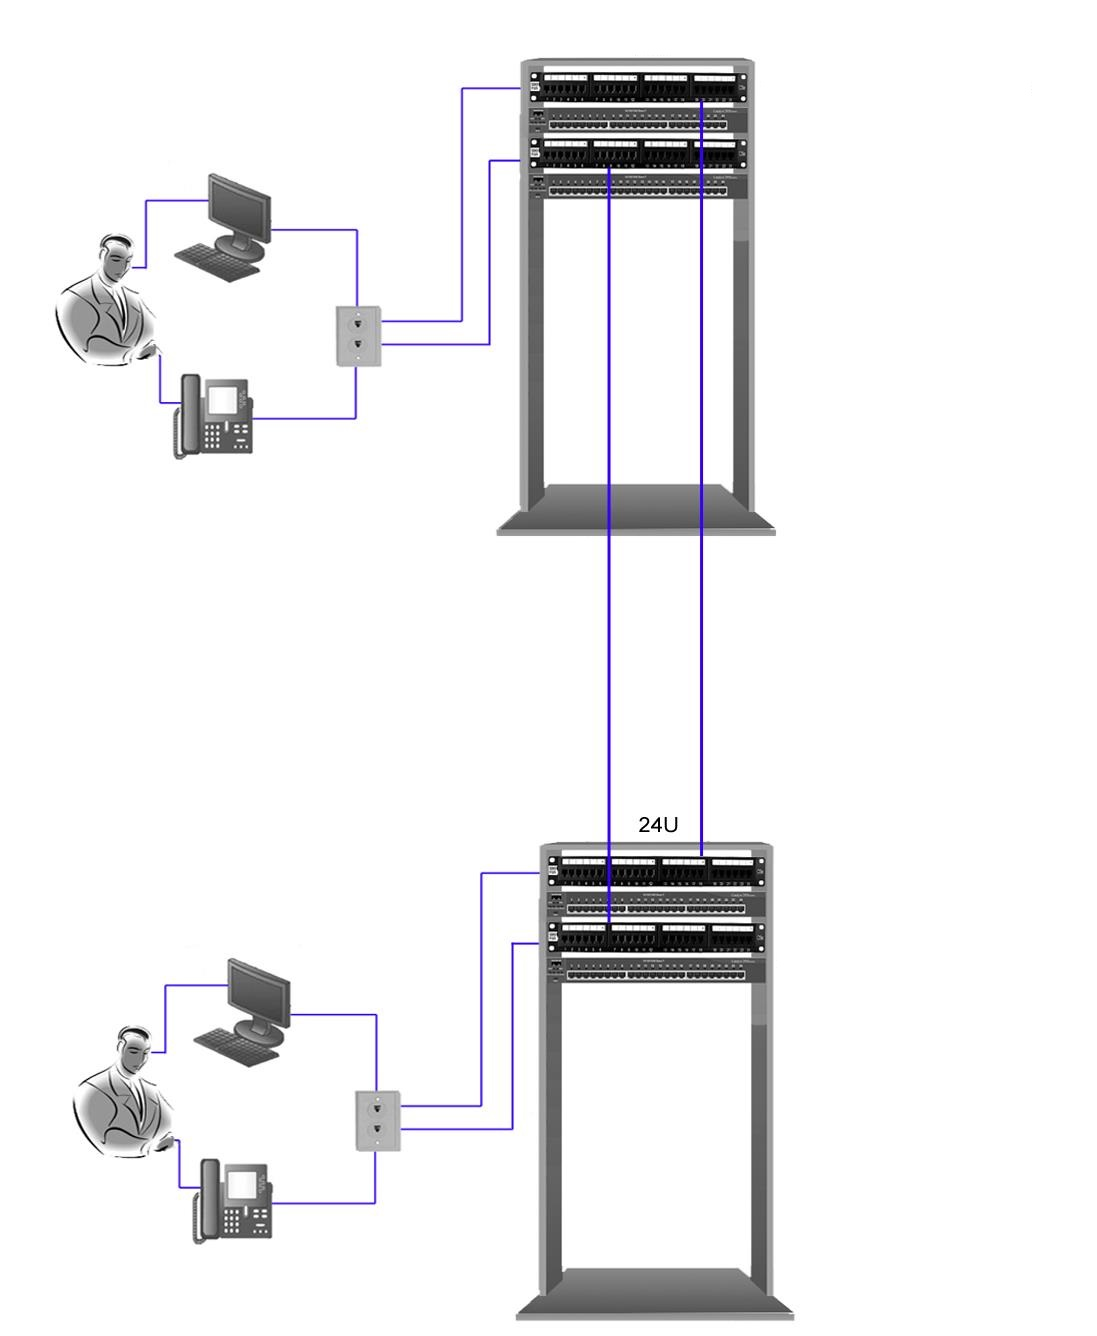
\includegraphics[width=\textwidth]{diagrama_logico}
	\caption{Diagrama da Rede}
	\label{diag_log}
\end{figure}
\FloatBarrier



\subsection{Encaminhamento}
Todo o cabeamento será realizado utilizando eletrocalhas em área aparente, todas as tomadas de telecomunicação que disponibilizam dados e voz estão a 45cm do chão conforme normas legais.

\subsection{Memorial descritivo}

Na Tabela \ref{equip} temos a lista de equipamentos e materiais utilizados para elaboração do projeto, a tabela também conta com informações de quantidade estimada e fabricante.

% Please add the following required packages to your document preamble:
% \usepackage{booktabs}
\begin{table}[]
\centering
\caption{Equipametos e Materiais Utilizados}
\label{equip}
\begin{tabular}{@{}|l|l|@{}}
\toprule
\textbf{Peça}                  & \textbf{Total} \\ \midrule
Organizador 1U                 & 8              \\ \midrule
Regua                          & 2              \\ \midrule
Tampa Plana Lisa               & 24.62          \\ \midrule
Caixa de derivação 1x1         & 24             \\ \midrule
RJ45 Krone                     & 48             \\ \midrule
Caixa de derivação 2X2         & 13             \\ \midrule
Duto Simples 45                & 84.18          \\ \midrule
Rack 24U 970mm                 & 2              \\ \midrule
Cabo lógico Categoria 6        & 817.90         \\ \midrule
Caixa de derivação 2X2         & 2              \\ \midrule
Painel Fechamento 1U           & 20             \\ \midrule
Tampa Plana Ranhurada          & 84.18          \\ \midrule
Estabilizador                  & 2              \\ \midrule
Switch 24 Portas               & 4              \\ \midrule
Caixa de derivação 2x2         & 24             \\ \midrule
Duto Canal                     & 25.64          \\ \midrule
Duto Simples 25                & 3              \\ \midrule
Patch Panel 24 Portas          & 4              \\ \midrule
Porta Equipamento 2 RJ45 Krone & 24             \\ \bottomrule
\end{tabular}
\end{table}
\FloatBarrier
\subsection{Identificação dos cabos}
A tabela \ref{pontos_p1} representa a identificação dos pontos das 6 salas presentes no piso 1.
A tabela \ref{pontos_p2} representa a identificação dos pontos das 9 salas presentes no piso 2, com a seguinte legenda:
\begin{itemize}
	\item TO - Número da tomada de telecomunicação
	\item A  - Patch Panel - Dados
	\item B  - Patch Panel - Voz
	\item SL - Sala 
	\item P  - Piso
\end{itemize}

\begin{table}[]
	\centering
	\caption{Identificação Pontos Piso 1}
	\label{my-label}
	\begin{tabular}{cccc}
		\hline
		\textbf{LOCAL}  & \textbf{SERVIÇO} & \textbf{IP} & \textbf{PORTA/PONTO} \\ \hline
		Sala 1          & Dados            & 172.17.0.2  & TO1ASL1P1            \\ \hline
		Sala 1          & Voz              & 10.10.12.2  & TO1BSL1P1            \\ \hline
		Sala 1          & Dados            & 172.17.0.3  & TO2ASL1P1            \\ \hline
		Sala 1          & Voz              & 10.10.12.3  & TO2BSL1P1            \\ \hline
		Sala 1          & Dados            & 172.17.0.4  & TO3ASL1P1            \\ \hline
		Sala 1          & Voz              & 10.10.12.4  & TO3BSL1P1            \\ \hline
		Sala 2          & Dados            & 172.17.0.5  & TO4ASL2P1            \\ \hline
		Sala 2          & Voz              & 10.10.12.5  & TO4BSL2P1            \\ \hline
		Sala 2          & Dados            & 172.17.0.6  & TO5ASL2P1            \\ \hline
		Sala 2          & Voz              & 10.10.12.6  & TO5BSL2P1            \\ \hline
		Sala 3          & Dados            & 172.17.0.7  & TO6ASL3P1            \\ \hline
		Sala 3          & Voz              & 10.10.12.7  & TO6BSL3P1            \\ \hline
		Sala 4          & Dados            & 172.17.0.8  & TO7ASL4P1            \\ \hline
		Sala 4          & Voz              & 10.10.12.8  & TO7BSL4P1            \\ \hline
		Sala 4          & Dados            & 172.17.0.9  & TO8ASL4P1            \\ \hline
		Sala 4          & Voz              & 10.10.12.9  & TO8BSL4P1            \\ \hline
		Sala 4          & Dados            & 172.17.0.10 & TO9ASL4P1            \\ \hline
		Sala 4          & Voz              & 10.10.12.10 & TO9BSL4P1            \\ \hline
		Sala 4          & Dados            & 172.17.0.11 & TO10ASL4P1           \\ \hline
		Sala 4          & Voz              & 10.10.12.11 & TO10BSL4P1          \\ \hline
		Sala 5          & Dados            & 172.17.0.12 & TO11ASL5P1           \\ \hline
		Sala 5          & Voz              & 10.10.12.12 & TO11BSL5P1           \\ \hline
		Sala 5          & Dados            & 172.17.0.13 & TO12ASL5P1           \\ \hline
		Sala 5          & Voz              & 10.10.12.13 & TO12BSL5P1           \\ \hline
		Sala 5          & Dados            & 172.17.0.14 & TO13ASL5P1           \\ \hline
		Sala 5          & Voz              & 10.10.12.14 & TO13BSL5P1           \\ \hline
		Sala 5          & Dados            & 172.17.0.15 & TO14ASL5P1           \\ \hline
		Sala 5          & Voz              & 10.10.12.15 & TO14BSL5P1           \\ \hline
	\end{tabular}
\end{table}
\FloatBarrier
\begin{table}[]
\centering
\caption{Identificação Pontos Piso 2}
\label{pontos_p2}
\begin{tabular}{cccc}
\hline
\textbf{LOCAL}  & \textbf{SERVIÇO} & \textbf{IP} & \textbf{PORTA/PONTO} \\ \hline
Sala 2          & Dados            & 172.17.0.16 & TO1ASL1P2            \\ \hline
Sala 2          & Voz              & 10.10.12.16 & TO1BSL1P2            \\ \hline
Sala 2          & Dados            & 172.17.0.17 & TO2ASL1P2            \\ \hline
Sala 2          & Voz              & 10.10.12.17 & TO2BSL1P2            \\ \hline
Sala 2          & Dados            & 172.17.0.18 & TO3ASL1P2            \\ \hline
Sala 2          & Voz              & 10.10.12.18 & TO3BSL1P2            \\ \hline
Sala 3          & Dados            & 172.17.0.19 & TO4ASL2P2            \\ \hline
Sala 3          & Voz              & 10.10.12.19 & TO4BSL2P2            \\ \hline
Sala 3          & Dados            & 172.17.0.20 & TO5ASL2P2            \\ \hline
Sala 3          & Voz              & 10.10.12.20 & TO5BSL2P2            \\ \hline
Sala 3          & Dados            & 172.17.0.21 & TO6ASL3P2            \\ \hline
Sala 3          & Voz              & 10.10.12.21 & TO6BSL3P2            \\ \hline
Sala 6          & Dados            & 172.17.0.22 & TO7ASL4P2            \\ \hline
Sala 6          & Voz              & 10.10.12.22 & TO7BSL4P2            \\ \hline
Sala 6          & Dados            & 172.17.0.23 & TO8ASL4P2            \\ \hline
Sala 6          & Voz              & 10.10.12.23 & TO8BSL4P2            \\ \hline
Sala 7          & Dados            & 172.17.0.24 & TO9ASL4P2            \\ \hline
Sala 7          & Voz              & 10.10.12.24 & TO9BSL4P2            \\ \hline
Sala 7          & Dados            & 172.17.0.25 & TO10ASL4P2           \\ \hline
Sala 7          & Voz              & 10.10.12.25 & TO10BSL4P2           \\ \hline
\end{tabular}
\end{table}
\FloatBarrier
\section{Implantação}
A imagem \ref{cron} indica o cronograma para execução das etapas do projeto de cabeamento estruturado, desde a demarcação dos pontos até a finalização do projeto.

\begin{figure}[h!]
	\centering
	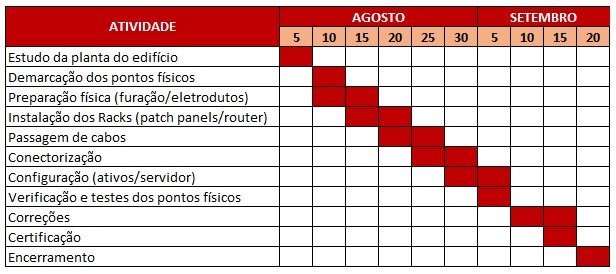
\includegraphics[width=\textwidth]{cronograma}
	\caption{Cronograma de Implementação}
	\label{cron}
\end{figure}

\section{Plano de certificação}
A certificação será executada por empresa diferente da executante do projeto no intuito de aumentar a confiabilidade dos testes executados no cabeamento;\newline
A certificação deverá ser executada preferencialmente na modalidade “Link permanente”;\newline
Ao final da certificação deverá ser entregue relatório final da certificação para cada ponto/segmento testado, constando o resultado do teste para cada parâmetro indicado;\newline
Os testes de 100\% dos segmentos de cabos deverão ser adotados os seguintes parâmetros de teste:\newline
\begin{itemize}
	\item Inspeção Visual; 
	\item Wire Map; 
	\item Comprimento; 
	\item Atenuação; 
	\item Resistência e Capacitância; 
	\item Next;
	\item PSNext; 
	\item Return Loss; 
	\item Fext; 
	\item Elfext; 
	\item PSELfext; 
	\item Propagation Delay; 
	\item Delay Skew. 
	\item  A Certificação de 100\% dos segmentos, de conformidade com as normas para a CATEGORIA 6;
\end{itemize}
\section{Plano de manutenção}

A manutenção será realizada a cada 3 meses nos dois primeiros anos e a cada 6 meses posteriormente, Serão realizadas trocas de componentes defeituosos decorrente de problemas de fabricação por um período de 5 anos. Visitas extras serão solicitadas até em 5 dias úteis após a solicitação do contratante.

\subsection{Plano de expansão}
Existe um projeto de expansão no que diz respeito a criação de um laboratório de informática na escola para realizar treinamentos na área de TI, na infraestrutura proposta é possível o aumento de 14 pontos de dados e 14 pontos de voz para o piso 1 e aumento de 9 pontos de dados e 9 de voz para o piso 2.

%\section{Risco}
%Apresentar os riscos do projeto

\section{Orçamento}
A tabela \ref{orc} apresenta o orçamento dos materiais e serviço de mão obra, a referente valor já engloba os custos com a certificação.

\begin{table}[h!]
\centering
\caption{Orçamento Materiais e Mão de Obra}
\label{orc}
\begin{tabular}{|l|l|l|l|l|}
\hline
\multicolumn{1}{|c|}{\textbf{Peça}} & \multicolumn{1}{c|}{\textbf{Marca}} & \multicolumn{1}{c|}{\textbf{Total}} & \multicolumn{1}{c|}{\textbf{Valor}} & \multicolumn{1}{c|}{\textbf{Valor Total}} \\ \hline
Organizador 1U                      & Furukawa                            & 8 Unidade                           & R\$      19,90                      & R\$     159,20                            \\ \hline
Regua                               & Furukawa                            & 2 Unidade                           & R\$    140,00                       & R\$     280,00                            \\ \hline
RJ45                                & Furukawa                            & 48 Unidade                          & R\$      29,00                      & R\$  1.392,00                             \\ \hline
Rack 24U 970mm                      & Furukawa                            & 2 Unidade                           & R\$ 1.087,90                        & R\$  2.175,80                             \\ \hline
Cabo lógico Categoria 6             & Furukawa                            & 3 Caixas                            & R\$    807,90                       & R\$  2.423,70                             \\ \hline
Painel Fechamento 1U                & Furukawa                            & 20 Unidade                          & R\$        7,00                     & R\$     140,00                            \\ \hline
Nobreak                             & APC                                 & 2 Unidade                           & R\$ 1.997,90                        & R\$   3.995,80                            \\ \hline
Switch 24 Portas                    & Cisco                               & 4 Unidade                           & R\$ 6.999,00                        & R\$ 27.996,00                             \\ \hline
Patch Panel 24 Portas               & Furukawa                            & 4 Unidade                           & R\$    503,77                       & R\$ 2.015,08                              \\ \hline
Mão de Obra                         &                                     &                                     &                                     & R\$ 10.000,00                             \\ \hline
\textbf{Total}                      &                                     &                                     &                                     & \textbf{R\$ 50.577,58}                    \\ \hline
\end{tabular}
\end{table}

%\section{Recomendações}
%Observações e recomendações para o cliente.

\section{Referências bibliográficas}
\begin{itemize}
	\item ASSOCIAÇÃO BRASILEIRA DE NORMAS TÉCNICAS. NBR 14565: Procedimento básico para elaboração de projetos de cabeamento de telecomunicações para rede interna estruturada. Rio de Janeiro: Abnt – Associação Brasileira de Normas Técnicas, 2000. 48 p.
	
	\item MARIN, Paulo Sérgio. Cabeamento Estruturado: Desenvolvendo cada passo: do projeto à instalação. 3. ed. São Paulo: Érica Ltda., 2010. 336 p.
	
	\item TELECOMMUNICATIONS INDUSTRY ASSOCIATION / ELECTRONIC INDUSTRIES ALLIANCE. 568-B.1-2001: Commercial Building Telecommunications Cabling Standard. Arlington, Va, Estados Unidos: Telecommunications Industry Association 2001, 2001. 79 p.
	
\end{itemize}
\end{document}